\begin{figure}[tb]
\internal{}
\setfigname{}
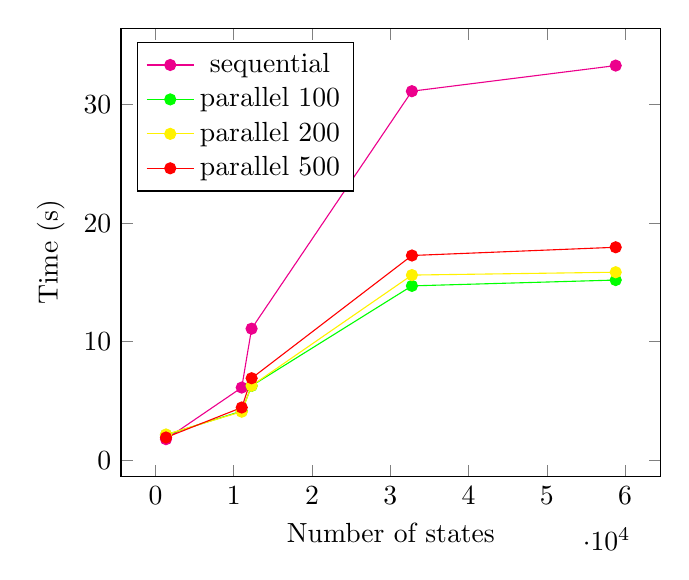
\begin{tikzpicture}
\definecolor{color0}{rgb}{0.75,0,0.75}

\begin{axis}[legend style={legend pos=north west},
ylabel={Time (s)},
xlabel={Number of states},
legend entries={{sequential},{parallel 100},{parallel 200},{parallel 500}}
% scaled ticks=false
]

% Sequential
\addplot [magenta, mark=*, mark size=2pt]
coordinates {
(1350,    1.783922000)
(11025,   6.135198000)
(12284,  11.098990000)
(32762,  31.121684000)
(58800,  33.280614000)
};

% 100
\addplot [green, mark=*, mark size=2pt]
coordinates {
(1350,   2.141683000)
(11025,  4.152756000)
(12288,  6.279725000)
(32768, 14.708286000)
(58800, 15.199168000)
};

% 200
\addplot [yellow, mark=*, mark size=2pt]
coordinates {
(1350,   2.177722000)
(11025,  4.099828000)
(12288,  6.293006000)
(32768, 15.619113000)
(58800, 15.858879000)
};

% 500
\addplot [red, mark=*, mark size=2pt]
coordinates {
(1350,   1.926380000)
(11025,  4.453230000)
(12288,  6.920561000)
(32768, 17.269375000)
(58800, 17.962744000)
};


\end{axis}
\end{tikzpicture}
\caption{A comparison between the run-times of PIPE 5's sequential state space exploration algorithm and the new MapReduce-style parallel algorithm running on 4 cores. We have allowed the parallel implementation to explore 500, 200, and 100 states before the reduction phase of each iteration. All parallel implementations yield at least a 2x speedup over the sequential algorithm although the 100 states per thread run performs slightly better than the others.}
\label{fig:parallel_vs_sequential_algo}
\end{figure}